\documentclass{article}\usepackage[]{graphicx}\usepackage[]{xcolor}
% maxwidth is the original width if it is less than linewidth
% otherwise use linewidth (to make sure the graphics do not exceed the margin)
\makeatletter
\def\maxwidth{ %
  \ifdim\Gin@nat@width>\linewidth
    \linewidth
  \else
    \Gin@nat@width
  \fi
}
\makeatother

\definecolor{fgcolor}{rgb}{0.345, 0.345, 0.345}
\newcommand{\hlnum}[1]{\textcolor[rgb]{0.686,0.059,0.569}{#1}}%
\newcommand{\hlsng}[1]{\textcolor[rgb]{0.192,0.494,0.8}{#1}}%
\newcommand{\hlcom}[1]{\textcolor[rgb]{0.678,0.584,0.686}{\textit{#1}}}%
\newcommand{\hlopt}[1]{\textcolor[rgb]{0,0,0}{#1}}%
\newcommand{\hldef}[1]{\textcolor[rgb]{0.345,0.345,0.345}{#1}}%
\newcommand{\hlkwa}[1]{\textcolor[rgb]{0.161,0.373,0.58}{\textbf{#1}}}%
\newcommand{\hlkwb}[1]{\textcolor[rgb]{0.69,0.353,0.396}{#1}}%
\newcommand{\hlkwc}[1]{\textcolor[rgb]{0.333,0.667,0.333}{#1}}%
\newcommand{\hlkwd}[1]{\textcolor[rgb]{0.737,0.353,0.396}{\textbf{#1}}}%
\let\hlipl\hlkwb

\usepackage{framed}
\makeatletter
\newenvironment{kframe}{%
 \def\at@end@of@kframe{}%
 \ifinner\ifhmode%
  \def\at@end@of@kframe{\end{minipage}}%
  \begin{minipage}{\columnwidth}%
 \fi\fi%
 \def\FrameCommand##1{\hskip\@totalleftmargin \hskip-\fboxsep
 \colorbox{shadecolor}{##1}\hskip-\fboxsep
     % There is no \\@totalrightmargin, so:
     \hskip-\linewidth \hskip-\@totalleftmargin \hskip\columnwidth}%
 \MakeFramed {\advance\hsize-\width
   \@totalleftmargin\z@ \linewidth\hsize
   \@setminipage}}%
 {\par\unskip\endMakeFramed%
 \at@end@of@kframe}
\makeatother

\definecolor{shadecolor}{rgb}{.97, .97, .97}
\definecolor{messagecolor}{rgb}{0, 0, 0}
\definecolor{warningcolor}{rgb}{1, 0, 1}
\definecolor{errorcolor}{rgb}{1, 0, 0}
\newenvironment{knitrout}{}{} % an empty environment to be redefined in TeX

\usepackage{alltt}
\usepackage{amsmath} %This allows me to use the align functionality.
                     %If you find yourself trying to replicate
                     %something you found online, ensure you're
                     %loading the necessary packages!
\usepackage{amsfonts}%Math font
\usepackage{graphicx}%For including graphics
\usepackage{hyperref}%For Hyperlinks
\usepackage[shortlabels]{enumitem}% For enumerated lists with labels specified
                                  % We had to run tlmgr_install("enumitem") in R
\hypersetup{colorlinks = true,citecolor=black} %set citations to have black (not green) color
\usepackage{natbib}        %For the bibliography
\setlength{\bibsep}{0pt plus 0.3ex}
\bibliographystyle{apalike}%For the bibliography
\usepackage[margin=0.50in]{geometry}
\usepackage{float}
\usepackage{multicol}

%fix for figures
\usepackage{caption}
\newenvironment{Figure}
  {\par\medskip\noindent\minipage{\linewidth}}
  {\endminipage\par\medskip}
\IfFileExists{upquote.sty}{\usepackage{upquote}}{}
\begin{document}

\vspace{-1in}
\title{Lab XX -- MATH 240 -- Computational Statistics}

\author{
  Charles Hooey \\
  Colgate University  \\
  Mathematical Economics Major  \\
  {\tt chooey@colgate.edu}
}

\date{}

\maketitle

\begin{multicols}{2}
\begin{abstract}
This assignment explores the various statistical components beta distribution through the graphical summarization of each component, and analysis of how each population level statistic compares with cumulative statistics sourced from randomly generated data from a known distribution. We then derived the moments of the beta distribution, and used them to compute the population level statistics, and create MOM and MLE point estimator functions. After comparing the graphs and statistics from each parameter obtained from our estimator functions, we concluded that the MLE was the more accurate estimator of the alpha and beta parameters for modeling a distribution with unknown parameters. 
\end{abstract}

\noindent \textbf{Keywords:} Point Estimation, Probability Density Function, Parameters

\section{Introduction}
This laboratory assignment aims to interact with and explore the behavior of the beta distribution. First, we aim to examine how statistical measurements are derived from this distribution, and how their behavior on the population level compares with randomly simulated data from a known distribution with the same parameters. We also seek to better understand the moments of the beta distribution, and how these are used to derive the mean, variance, skewness and kurtosis of a data set. Following this, we seek to determine an efficient way of finding which values of alpha and beta may be used to model a particular set of data, and consequently, determine the most accurate and representative method of point estimation.


\section{Density Functions and Parameters}
As mentioned before, this laboratory assignment was aimed at deepening our understanding of and strengthening our ability to interact with the beta distribution. Being a continuous distribution, we first interpreted the behavior of the beta distribution through examining how its parameters of alpha and beta dictate the shape of the distribution's probability density function. To do such, we analyzed the beta distribution with four different combinations of the alpha and beta parameters:
\begin{itemize}\itemsep0em
\item $\alpha = 2, \beta = 5$
\item $\alpha = 5, \beta = 5$
\item $\alpha = 5, \beta = 2$
\item $\alpha = 0.5, \beta = 0.5$
\end{itemize}


After computing the numerical summary for each of the distributions, we graphed them each with a density plot and superimposed a normal distribution with the same mean and variance to observe the differences between the two as the shape of the beta distribution changes. Comparing all four graphs of the distributions led us to make an assumption that a negative difference between alpha and beta leads to the distribution being more right skewed while a positive difference reflected the opposite. When the two are the same, the data has a skewness of zero. The statistics for each of the parameter combinations are given in the following table:

% latex table generated in R 4.4.2 by xtable 1.8-4 package
% Tue Apr  1 20:54:00 2025
\begin{table}[H]
\centering
\begingroup\small
\begin{tabular}{rrrrrr}
  \hline
alpha & beta & mean & variance & skewness & kurtosis \\ 
  \hline
2.00 & 5.00 & 0.29 & 0.03 & 0.60 & -0.12 \\ 
  5.00 & 5.00 & 0.50 & 0.02 & 0.00 & -0.46 \\ 
  5.00 & 2.00 & 0.71 & 0.03 & -0.60 & -0.12 \\ 
  0.50 & 0.50 & 0.50 & 0.12 & 0.00 & -1.50 \\ 
   \hline
\end{tabular}
\endgroup
\label{beta_table}
\end{table}



\section{Properties of the Beta Distribution}
The statistical components of the beta distribution that we analyzed were its mean, variance, skewness and kurtosis. To calculate the statistics of the four pairs of beta distribution parameters we had analyzed numerically and graphically, we first used formulas that were strictly dependent on the parameters alpha and beta. For the second task of this lab, however, we obtained these statistical measurements using the centered and uncentered moments of the beta distribution, which all of the statistics of interest are comprised of. When comparing the values obtained by using the moments to the measurements found with the alpha and beta parameter formulas, we observed that each measurement is almost exactly the same as its respective counterpart. 

\subsection{Random Data Sampling}
The third task of this assignment was to explore how the population statistics of our data would compare with statistics drawn from a generated and known distribution. To accomplish such, we used R to generate a sample beta distribution of size n = 500 for each of the four parameter combinations we were originally working with. The statistics calculated for each of the distributions were close but not the exact same as our original population level. Furthermore, the plots shared the same visual features as the ones that were created within task one, as the skewness and mean of each were close to one another for each respective combination of parameters.

\subsection{Behavior of Cumulative Statistics}
Task four of this lab involved examining the behavior of cumulative statistics across many different generated beta distributions of the same parameters (alpha = 2, beta = 5). We used loops and the \texttt{cumstats} package for \texttt{R} to accomplish this, then plotted the original beta distribution and superimposed lines of different colors for each randomly generated statistic \citep{cumstats}. After observing the graphical behavior of each of the statistics, the randomly generated beta distribution statistics suggest that the cumulative statistics for this distribution will all converge to the same value as one another. Task five additionally had us use loops to generate 1000 random samples of size n = 500 for the beta distribution and to graphically summarize each statistic by plotting their distributions. Each of the statistics' distributions were centered almost exactly at their respective population statistic values, which suggests that the cumulative statistics for randomly generated samples should converge to the population level statistics if the sample size is adequate.

\section{Point Estimation}
Task six of this assignment had us explore how country death rates could be modeled with the beta distribution. Because the support of the beta distribution was 0 to 1, it was first necessary to use the \texttt{Tidyverse} package for \texttt{R} to wrangle the data and convert each value into a rate over 1000 \citep{tidyverse}. following such, we created two functions that would estimate the values of alpha and beta through two different types of point estimation: Method of Moments and Maximum Likeliness. After creating a function for and plotting the distributions resulting from the MOM and MLE point estimators, the results both were concurrent with the histogram of the data, and were almost identical with one another, as seen in figure \ref{fig1}. This suggests that both methods of point estimation provided values for alpha and beta that were close to the true values for the distribution of the data.

\begin{figure}[H]
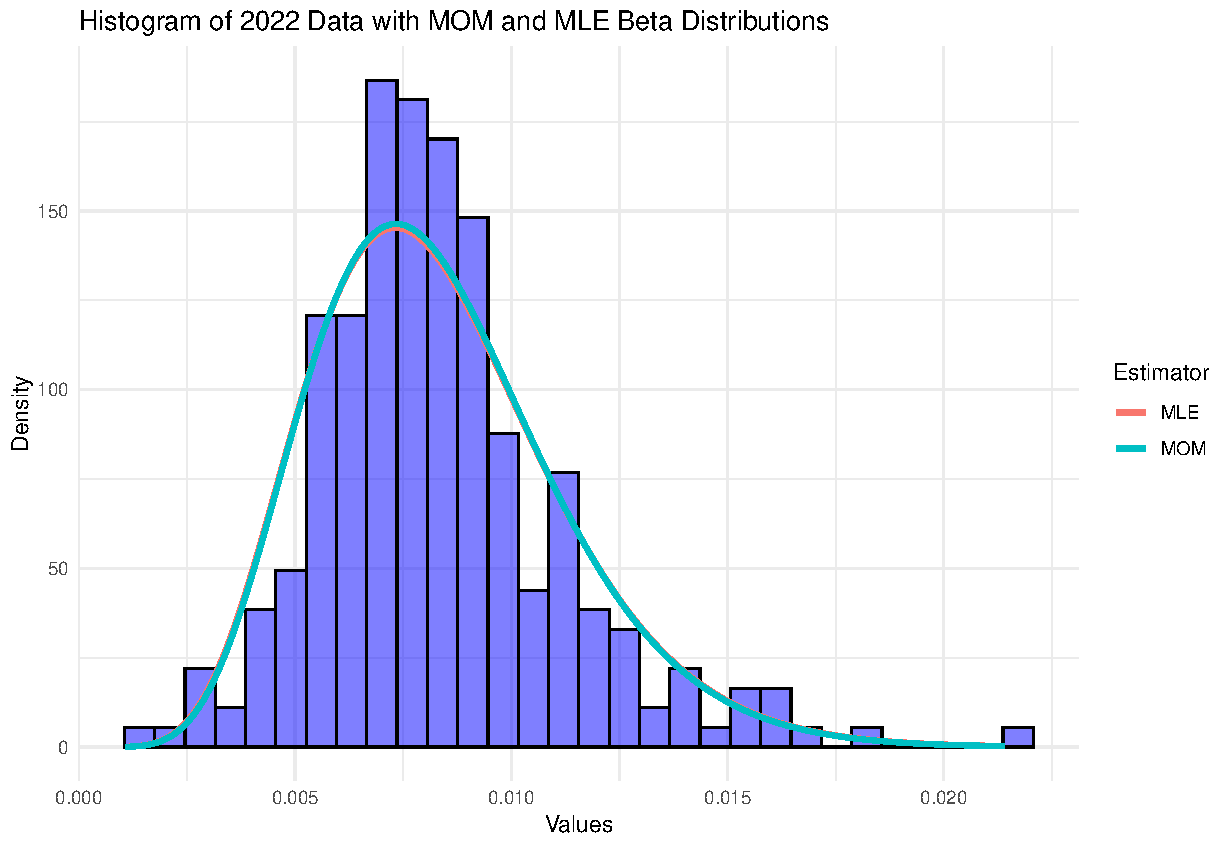
\includegraphics[scale=0.4]{Ptestdist.pdf}
\caption{Histogram of Death Rates with MOM and MLE Distributions Superimposed}
\label{fig1}
\end{figure}

\subsection{MOM and MLE Estimators}
After working with the death rate data provided, we pivoted to once again use loops to simulate data, this time in order to compare the distribution of parameters obtained from each method of point estimation. For these calculations, we used values of alpha = 8, beta = 950, and n = 266. In order to make a conclusion on the best estimator for the alpha and beta parameters, we graphed the distribution for each parameter, and calculated their respective bias, precision, and mean square error. Comparing the results from the MOM and MLE estimators provided evidence towards MLE being the more accurate point estimator, as it held a lower bias and higher precision than the MOM, and visually, as observed within figure \ref{fig2}, appeared to follow the histogram of the data more closely than the plot of the MOM distribution did.

\begin{figure}[H]
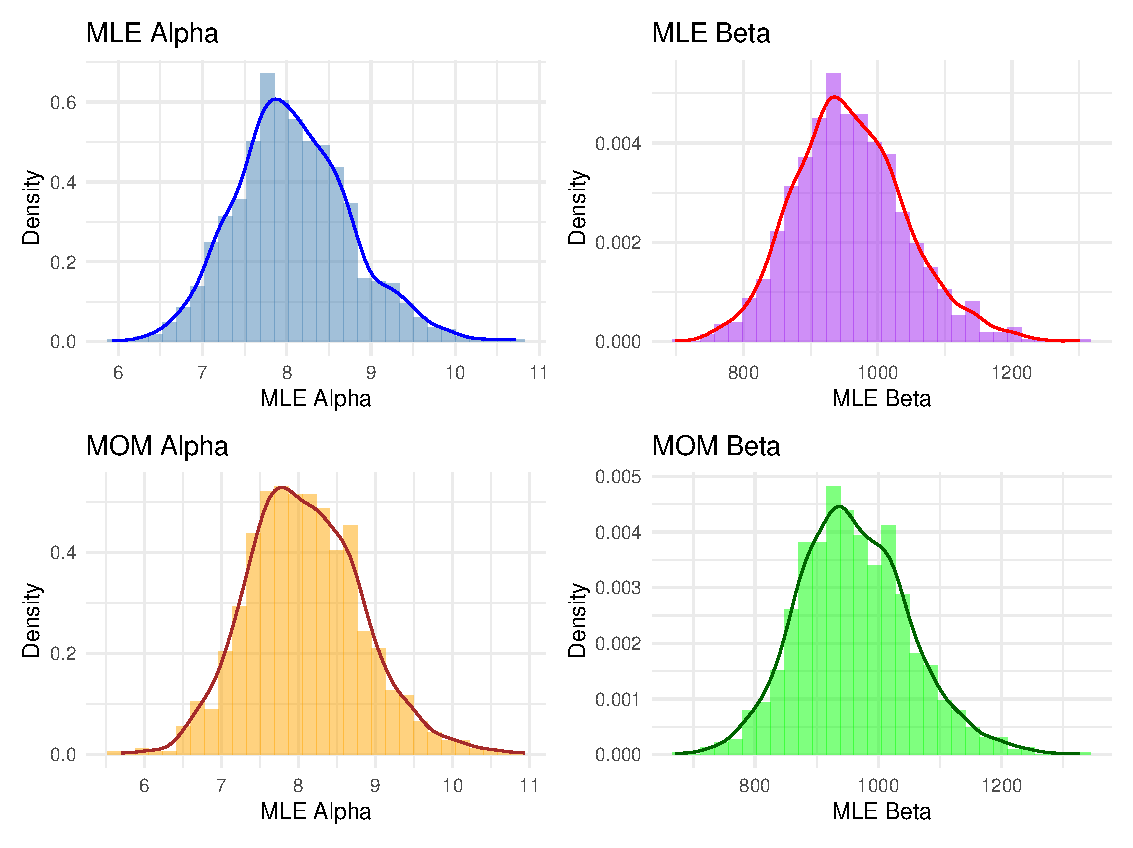
\includegraphics[scale=0.4]{ptestgraph.pdf}
\caption{Estimated Probability Distributions for MOM and MLE Parameters}
\label{fig2}
\end{figure}


%%%%%%%%%%%%%%%%%%%%%%%%%%%%%%%%%%%%%%%%%%%%%%%%%%%%%%%%%%%%%%%%%%%%%%%%%%%%%%%%
% Bibliography
%%%%%%%%%%%%%%%%%%%%%%%%%%%%%%%%%%%%%%%%%%%%%%%%%%%%%%%%%%%%%%%%%%%%%%%%%%%%%%%%
\vspace{2em}

\noindent\textbf{Bibliography:}


\begin{tiny}
\bibliography{bib}
\end{tiny}
\end{multicols}
\end{document}
%%%%%%%%%%%%%%%%%%%%%%%%%%%%%%%%%%%%%%%%%%%%%%%%%%%%%%%%%%%%%%%%%%%%%%%%%%%%%%%%
% Appendix
%%%%%%%%%%%%%%%%%%%%%%%%%%%%%%%%%%%%%%%%%%%%%%%%%%%%%%%%%%%%%%%%%%%%%%%%%%%%%%%%




